\section{Principle}




Our flexible fish-eye based lens consists in modifying the rays (origin and direction) which cross the subset of the volume located under this lens.
Our volume rendering framework relies on a GPU accelerated ray-casting algorithm. The basic idea of GPU-based ray-casting is to store the dataset into a 3D texture, and run a compute kernel that casts rays through this volume. Each pixel of the output image corresponds to the compositing of all sampled data along a single ray of sight. In classic ray-casting algorithms (\autoref{f:fisheye}-a), each ray is a line defined by the eye position $e$ or the camera which is the same for all rays, and a normalized direction vector $\vec{d}\left(x,y\right)$  where $x$ and $y$ are the screen space coordinates of the pixel. The position of each sample along a single ray is then $\vec{p}\left(x,y,t\right) = \vec{e} + t \times \vec{d}\left(x,y\right)$ with $t \in \left[t_{near},t_{far}\right]$ , where $t$ represents the depth or basically the distance between the eye and the sample which varies from the distance where the ray meets the volume $t_{near}$ to the distance where the ray leaves the volume $t_{far}$.
Our circular lens modifies the behavior of all the rays that travel through it in order to magnify a target. The new ray behavior can be divided into 3 steps. The first step is to provide an unobstructed view. It consists of moving closer to the target while avoiding the obstacles and pushing them aside. The second step is to set a wider field of view (fish-eye) in order to see most of the target. The last step which is optional offers a set of interaction to modify some visual parameters in real time such as the rays orientation and the field of view.

\subsection{Setting an unobstructed view }
While exploring a volumetric dataset, people want to have more details and information on items which are partially visible because of the occlusion created by other items in front of them. The aim of this step is to provide an unobstructed view by moving closer to the target while avoiding the obstacles and pushing them aside.
Getting closer to the target can be carried out automatically or manually. When the user selects an occluded target, the rays traveling through the lens will share the same constant direction $\vec{d}_{target}$ inside the volume until they reach same the depth $t_{target}$ near the selected target. By default, this direction  $\vec{d}_{target}$ goes straight towards the selected item (the focal point $\vec{p}_{target}$). A sampled value inside the dataset located before the target has a position $\vec{p}$ defined by $\vec{p}\left(x,y,t\right) = \vec{p}_{near}\left(x,y\right) + t \times \vec{d}_{target}$ where $\vec{p}_{near}\left(x,y\right)$ is the point where the ray meets the volume while following is initial direction $\vec{d}\left(x,y\right)$. In addition to getting closer to the target, this new rays' direction also allows magnifying the subset of the volume located below the lens. In fact, inside the volume, these rays become parallel and converge toward the axis of the lens. This behavior creates a magnification below the lens (\autoref{f:fisheye}-b). 

Moreover, we offer the possibility to describe manually the ray trajectory inside the volume. In this case the rays' trajectories are parallel curves going through the volume towards a selected location. The direction $\vec{d}_{target}\left(t\right)$ associates a normalized vector indicating a location to a depth $t$ according to the user inputs. The position of a sampled value inside the volume is then: $\vec{p}\left(x,y,t\right) = \vec{p}_{near}\left(x,y\right) + t \times \vec{d}_{target}\left(t\right)$.

After the previous step, the rays are close to the target which can still be occluded. To address this issue, we introduced a radial attraction force for each ray which goes from the initial ray position after the previous step to the center of the lens. The new position of a sample point can be defined as $\vec{p}\left(x,y,t\right) = \vec{p}_{near}\left(x,y\right) + t \times \vec{d}_{target} + a \times \vec{f}_{attraction} $ with $a \in \left[0,1\right]$ which represents the attraction factor. When $a$ is close to $0$ the rays follow their initial parallel directions, and conversely when $a$ is close to $1$ the rays follow the same trajectory which is the axis of the lens (when the trajectory was set automatically) or the curve designed by the user. During this step, attracting all the ray inside the lens towards a single trajectory allows pushing aside the obstacles around this trajectory.  
However, these new trajectories create discontinuities at the lens border. We propose a solution in  section \ref{continuity} . 


\subsection{The field of view}
Once the rays of sight are close to the target, we are free from the obstacle but only see a small part of this target because of the zero distance between the rays. To address this issue, we propose to increase the field of view after the previous step. In fact, we diverge the rays which were previously sharing the same trajectory. Now, each ray is heading towards the outside of the lens according to the screen space coordinates of its corresponding pixel, as well as the angle of view. This wide angle of view (fish-eye) is by default set to $\alpha = 120^{\circ}$ instead of $180^{\circ}$ in order to keep the focus on the initial target because the rays can still be surrounded by other occluding items. The field of view can be adjusted by the user to have a better visibility of the target by using the scroll wheel while pressing the Shift key according to his/her desired action (\autoref{f:fisheye}-c).
\begin{figure} 
\includegraphics [width=0.45\textwidth]{images/bagage_orientation_bis.pdf} 
\caption{ A baggage presented under two different perspectives. (a) The baggage is composed by various type of items. the camera is located at the top front of the baggage. (b) The camera is located at the baggage side.  }
\label{f:baggage_orientation}
\end{figure}

\subsection{Interactive modification of the lens}
Our lens can be interactively modified in order to offer more flexibility thanks to a set of different parameters involved in both previous steps. The first editable parameter is the size of the lens. We opted for a circular shaped lens so its size is then decided by the radius that can be modified interactively by the user with the mouse wheel. The purpose is to provide an interactive focus+context tool. The bigger the radius is, the more the target inside the lens will be magnified. 

In addition, the trajectory which is automatically proposed after a target is selected can be modified by changing the location of the focal point $\vec{p}_{target}$ via the arrow keys. The final direction of the rays $\vec{d}_{target}$ can also be edited. This action can be carried out by a local rotation with the right button of the mouse. This allows adjusting the position of the rays near the target in a way to reduce the occlusion. Changing the directions of the rays can help to look around the target and get more information about its local context such the surrounding items and their relative positions.  

Furthermore, the factor applied to the radial attraction force $\vec{f}_{attraction}$  helps to push aside or reposition the occluding items located before the target by using the mouse wheel while holding the Shift key. This allows the user to restore the initial context at will, which can be very helpful to understand the actual configuration. By default, we set this attraction factor $a$ to the maximum $a=1$. In other terms, the rays follow the same trajectory as the axis of the lens. The new position of a sample point is defined as $\vec{p}\left(x,y,t\right) = \vec{p}_{near}\left(x,y\right) + t \times \vec{d}_{target} + \vec{f}_{attraction} $  in order to reduce the occlusion and provide an unobstructed view  on the selected target.

\subsection{Continuity and transitions}\label{continuity}

All the rays traveling through the lens have trajectories and behaviors very different from those which never cross this lens. Without any additional post-treatment, the previous steps create discontinuities at the boundary of the lens. To address this issue we use an interpolation function between the final ray trajectory and the one before the previous steps. In fact, the closer a ray is to the lens border, the closer is new trajectory will be to the previous one. This interpolation offers a smoother transition between the lens viewport and the rest of the volume. This linear interpolation $p\left(k\right)$ between the new position $p^{1}$ of a sample along the ray and the one if it was not modified by the lens $p^{0}$ can described as: $p\left(k\right) = p^{0} + f\left(k\right)\left( p^{1} - p^{0} \right)$ where $k \in  \left[0,1\right]$  is the normalized distance to the axis of the lens and $ f\left(k\right)\in  \left[0,1\right]$ is a function that modifies the speed of the interpolation. For instance, we used $ f\left(k\right) = k^2$ in order to reduce the interpolation near the center of the lens.
The algorithm \ref{alg:propagation} shows a pseudo code of the behavior of our deforming lens 


\begin{algorithm}
\SetKwInOut{Input}{Input}
\SetKwInOut{Output}{output}
\SetKwInOut{Parameter}{Parameter}

 \Input{
 $\vec{e}$: the eye position,
 
 $\vec{d}\left(x,y\right)$: the ray direction according to the screen space coordinates of the resulting pixel ($x$ and $y$),
 
 $step$: the sampling distance along the ray.
 
 }
 \KwResult{the pixel color.}
 
 \Parameter{
 $a$: the attraction factor,
 
 $\alpha$: the angle of view.
 }
\BlankLine
 
  $k  \leftarrow $ the normalized distance to the axis of the lens
 $\vec{p}_{near}  \leftarrow \vec{e} + t_{near} \times \vec{d}\left(x,y\right)$ //The initial position  \; 
 $\vec{p}^{0} \leftarrow \vec{p}_{near} $ \; 
 \While{ $ t \le t_{far}$ And $Opacity \le Opacity Threshold  $ }{
 	\If{the current ray is inside the lens}{
    	\If{ $t < t_{target}$ }{
        	$\vec{p}^{1} \leftarrow \vec{p}_{near}\left(x,y\right) + t \times \vec{d}_{target} + a \times \vec{f}_{attraction}$  \;
            \lElse{
        	$\vec{p}^{1} \leftarrow \vec{p}_{target} + \left( t-t_{target} \right) \times \vec{d}_{fishEye}\left( \alpha \right)$
        	}	
        }
               
    $\vec{p} \leftarrow \vec{p}^{0} + f\left(k\right) \times \left( \vec{p}^{1} - \vec{p}^{0} \right) $	\;
     \lElse{
     	 $\vec{p} \leftarrow \vec{p}^{0}$
     }
    }
\emph{Sampling at the position $\vec{p} $ }\;
    
    \emph{Shading the sampled value }\;
    
    \emph{ Compositing the shaded sampling point with the previous values} \;
 
    $t \leftarrow t + step$ \;
    $p^{0} \leftarrow p^{0} + step \times \vec{d}\left(x,y\right)$ \;

}
$color_{final} \leftarrow$ composited colors \;
return $color$
 

\label{alg:propagation}
 \caption{Pseudo code of our lens deformation algorithm}
\end{algorithm}


\begin{figure*} 
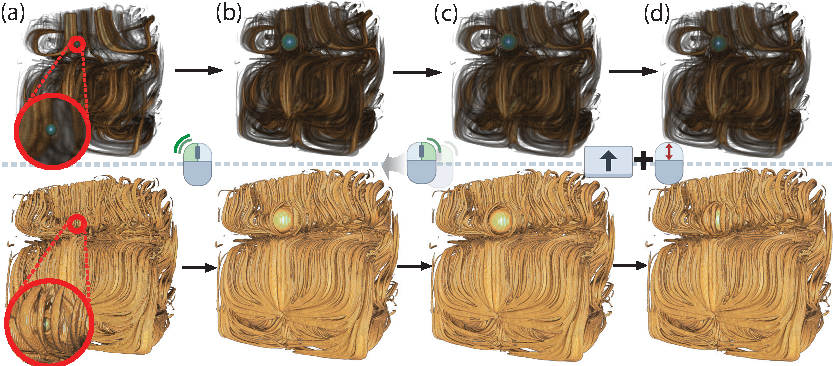
\includegraphics [width=\textwidth]{images/stream_lens.pdf} 
\caption{ A spherical item and its surrounding area are inspected using to our lens with 2 different transfer functions. The first part is displayed with transparency in opposition to the part below. The opacity helps to see the shape of the surrounding whirlpool. (a-a') The streamline dataset displayed using our framework. A dense object is hidden inside a whirlpool. (b-b') The lens tool is applied to the partially hidden object (double-click). The area is magnified and the occluding part of the whirlpool located in front of the spherical item is pushed aside. (c-c') The directions of the rays inside the lens are modified to see the whole sphere through the lens (right click+ mouse drag toward the desired direction). (d-d') The occluding part of the whirlpool can be restored/pushed gradually while keeping the area magnified (Shift + scroll).  }
\label{f:stream_lens}
\end{figure*}

\begin{figure} 
\includegraphics [width=0.45\textwidth]{images/streamline_orientation.pdf} 
\caption{ This figure shows 2 visualizations of a streamlines dataset. (a) The transfer function used allows to spot a spherical dense item inside the volume thanks to transparency. (b) This spherical object become occluded when the opacity of the surrounding whirlpool is increased in order to analyze its shape and behavior. }
\label{f:streamLineSTDViz}
\end{figure}
After the selection of a target, the lens offers a smooth transition between the previous view and the new one using a  slow-in/slow-out technique~\cite{Dragicevic:2011:TDA:1978942.1979233}. With this animation, the increase of the gradual speed at the beginning of the animation helps the user to start tracking the moving obstacles, and the decreasing speed at the end allows the user to predict where these occluding items stop moving. This also gives some semantic to the moving shapes, allowing the human mind to interpret the motion as a magnification of a target, and to keep the focus on visual entities during this transition. 

